% Options for packages loaded elsewhere
\PassOptionsToPackage{unicode}{hyperref}
\PassOptionsToPackage{hyphens}{url}
%
\documentclass[
  a4paper,
]{article}
\usepackage{amsmath,amssymb}
\usepackage{setspace}
\usepackage{iftex}
\ifPDFTeX
  \usepackage[T1]{fontenc}
  \usepackage[utf8]{inputenc}
  \usepackage{textcomp} % provide euro and other symbols
\else % if luatex or xetex
  \usepackage{unicode-math} % this also loads fontspec
  \defaultfontfeatures{Scale=MatchLowercase}
  \defaultfontfeatures[\rmfamily]{Ligatures=TeX,Scale=1}
\fi
\usepackage{lmodern}
\ifPDFTeX\else
  % xetex/luatex font selection
\fi
% Use upquote if available, for straight quotes in verbatim environments
\IfFileExists{upquote.sty}{\usepackage{upquote}}{}
\IfFileExists{microtype.sty}{% use microtype if available
  \usepackage[]{microtype}
  \UseMicrotypeSet[protrusion]{basicmath} % disable protrusion for tt fonts
}{}
\makeatletter
\@ifundefined{KOMAClassName}{% if non-KOMA class
  \IfFileExists{parskip.sty}{%
    \usepackage{parskip}
  }{% else
    \setlength{\parindent}{0pt}
    \setlength{\parskip}{6pt plus 2pt minus 1pt}}
}{% if KOMA class
  \KOMAoptions{parskip=half}}
\makeatother
\usepackage{xcolor}
\usepackage[margin=1in]{geometry}
\usepackage{graphicx}
\makeatletter
\def\maxwidth{\ifdim\Gin@nat@width>\linewidth\linewidth\else\Gin@nat@width\fi}
\def\maxheight{\ifdim\Gin@nat@height>\textheight\textheight\else\Gin@nat@height\fi}
\makeatother
% Scale images if necessary, so that they will not overflow the page
% margins by default, and it is still possible to overwrite the defaults
% using explicit options in \includegraphics[width, height, ...]{}
\setkeys{Gin}{width=\maxwidth,height=\maxheight,keepaspectratio}
% Set default figure placement to htbp
\makeatletter
\def\fps@figure{htbp}
\makeatother
\setlength{\emergencystretch}{3em} % prevent overfull lines
\providecommand{\tightlist}{%
  \setlength{\itemsep}{0pt}\setlength{\parskip}{0pt}}
\setcounter{secnumdepth}{-\maxdimen} % remove section numbering
\ifLuaTeX
\usepackage[bidi=basic]{babel}
\else
\usepackage[bidi=default]{babel}
\fi
\babelprovide[main,import]{catalan}
% get rid of language-specific shorthands (see #6817):
\let\LanguageShortHands\languageshorthands
\def\languageshorthands#1{}
\ifLuaTeX
  \usepackage{selnolig}  % disable illegal ligatures
\fi
\usepackage{bookmark}
\IfFileExists{xurl.sty}{\usepackage{xurl}}{} % add URL line breaks if available
\urlstyle{same}
\hypersetup{
  pdftitle={U3. WINDOWS SERVER. ADMINISTRACIÓ I CONFIGURACIÓ (V)},
  pdfauthor={@tofermos 2024},
  pdflang={ca-ES},
  hidelinks,
  pdfcreator={LaTeX via pandoc}}

\title{U3. WINDOWS SERVER. ADMINISTRACIÓ I CONFIGURACIÓ (V)}
\usepackage{etoolbox}
\makeatletter
\providecommand{\subtitle}[1]{% add subtitle to \maketitle
  \apptocmd{\@title}{\par {\large #1 \par}}{}{}
}
\makeatother
\subtitle{GESTIÓ DE UO I DIRECTIVES LOCALS DE SEGURETAT}
\author{@tofermos 2024}
\date{}

\begin{document}
\maketitle

{
\setcounter{tocdepth}{2}
\tableofcontents
}
\setstretch{1.5}
\newpage
\renewcommand\tablename{Tabla}

\section{1 Les UO}\label{les-uo}

Com ja hem explicat les UO són un objecte contenidor, d'ahi que es
representa al GUI amb una icona similar a la de els carpetes. El
contigut de les UO són altres objectes: usuaris, grups, carpetes
compartides i també altres UO.

\subsection{Per a què es creen les
UO?}\label{per-a-quuxe8-es-creen-les-uo}

Les UO són transparents a l'usuari. Un comptable pot detectar que forma
part d'alguna ``agrupació'' de companys del mateix despatx o continus i
intuir que són un ``grup'' d'usuaris. Però li costaria més intuir o
deduir la existència de UOs. De mode simplificat podríem dir que les UO
es creen per administrar la xarxa per parts. Per a que els
adminstradors, o usuaris avançats habilitats, puguen repartir-se la
faena d'administrar la xarxa sencera.

Els criteris o raons per crear UO poden ser tres:

1- Dividir l'administració del domini atenent a un \textbf{criteri
geogràfic}. Delegacions de països, zones\ldots{} o centres d producció
distints. 2- Dividir l'administració del domini atenent a un
\textbf{criteri organitzatiu}. Agrupant departaments de l'empresa, per
exemple. 3- Crear agrupacions d'objectes de forma \textbf{dinàmica} per
a projectes temporals. Una UO amb tots els recursos (objetes) per crear
una aplicació software nova, per desenvolupar un prjecte
urbanístics\ldots{}

\subsection{La divisió del treball duu
l'especialització}\label{la-divisiuxf3-del-treball-duu-lespecialitzaciuxf3}

El que està clar és que abandonem el paradigam de l'\emph{administrador
o administradors de tot el domini} i obrim les portes a que un usuari
(no necessàriament administrador) puga fer tasques (encara que bàsiques)
en el Servidor pròpies d'un administrador.

\section{2 La delegació de control de la
UO}\label{la-delegaciuxf3-de-control-de-la-uo}

Ja hem vist en aquesta unitat (U3.2) com es creen les UO i com es
modifiquen. Ara vorem com es delega el control en un usuari. Delegar el
control en un usuari Administrador del domini pot semblar un poc absurd;
interessa delegar en un altre tipus d'usuari que no siga Administrador
del tot per a convertir-lo en un ``quasi-administrador'' d'una part del
domini (la UO).

\subsubsection{Seleccionem l'usuari (o
usuaris)}\label{seleccionem-lusuari-o-usuaris}

Hem de buscar is seleccionar correctament l'usuari.

\begin{figure}
\centering
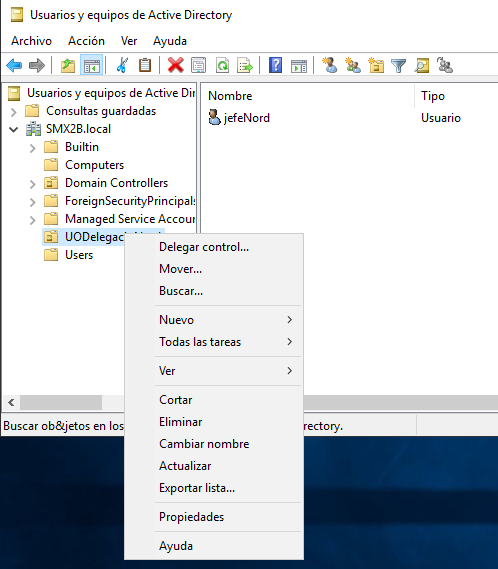
\includegraphics{png/DelegarControl1.png}
\caption{Delegar control}
\end{figure}

\subsubsection{Assignem drets}\label{assignem-drets}

\begin{figure}
\centering
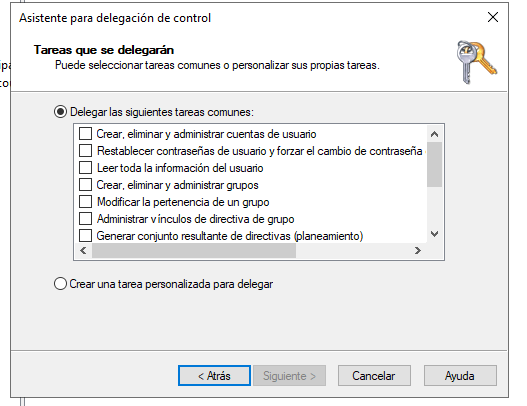
\includegraphics{png/DelegarControl2.png}
\caption{Assignar drets en al delegació}
\end{figure}

\end{document}
